\chapter{Neural Network}
Schaefer \etal \citeyear{schaefer_name_2011} were able to use the unique time course of the component responsible for the most variance to differentiate between stimuli.
With our components we were unable to reproduce this stimulus classification accuracy. 
 
To classify our data, we used a technique from the computer science called an artificial neural network (\ac{ANN}).
A neural network contains one or more layers that process the data.
In these layers, the input is processed by a filter (weight matrix) that is trained using backpropagation \cite{Rumelhart_backpropagation_1986}. 
Our network was optimized for our stimulus classification task and included three processing layers.
The first layer was pre-trained on the perception data using 432 trials (9 subjects x 12 stimuli x 4 trials) and then was not changed during training of the full 3-layer model. 
One trial of each stimulus from each subject's data was left out to be used as the test set for later model testing (108 trials (9 subjects x 12 stimuli x 1 trial) ).
The full explanation of how we arrived at the best model can be found in \cite{stober_ICLR2016} (arXiv:1511.04306).

\section{Layer 1: Similarity Constraint Encoding}
We wanted to find features in the data that were stable across trials and subjects, and also distinguished between classes. 
To identify such features, we used a pre-training strategy called \emph{similarity-constraint encoding}.
% in which the \ac{CAE} is trained to encode relative similarity constraints. 
As introduced by Schultz and Joachims \citeyear{schultz_learning_2004}, a relative similarity constraint $(a,b,c)$ describes a relative comparison of the trials $a$, $b$, and $c$ in the form ``$a$ is more similar to $b$ than $a$ is to $c$.''
Here, $a$ is the reference trial used for this comparison, $b$ is a trial from the same stimulus, and $c$ is a trial from another stimulus.
The number of violated constraints is used as a cost function for learning features of the data that are important for stimulus classification. 
A cost function describes the characteristics of the system that we want to minimize -- in this case we want to minimize the number of violations to the similarity constraint.

To this end, we combined all pairs of trials $(a,b)$ from the same stimulus with all trials $c$ from other stimuli.
During supervised learning, the system was forced to learn features of the data constrained by $a$ and $b$ being more similar than $a$ and $c$. 
For example, we created all possible pairs of trials from the perception of Jingle Bells with lyrics and then combined each of those pairs with all other perception trials.
Each one of these triplets was then processed by the \ac{SCE}. % (under the similarity constraint).
The \ac{SCE} learned features, in this case EEG channel weights, that, when applied to the EEG trials, produced representations of each one of the trials in the triplet. 
The representations were compared using the dot product as a similarity measure. 
Each triplet produced two similarity scores: one comparing $a$ and $b$ (trials from the same stimulus) and one comparing $a$ and $c$ (trials from different stimuli).
Based on our constraint, the similarity score between $a$ and $b$ must be higher than $a$ and $c$.

During training, the number of violated constraints was minimized using backpropagation and stochastic gradient descent with a learning rate momentum \cite{rumelhart1988learning}.
In this scenario, backpropagation allowed the \ac{SCE} to update its learned features (channel weights) to produce representations of the trials that satisfied the constraint. 
To help the \ac{SCE} hone in on the optimal learned features, stochastic gradient descent forced the learned features to be updated in the direction of minimizing the violations of the constraint. 
Learning rate momentum is a method for quickly achieving optimal results. Rather than the features (channel weights) being updated after each triplet was processed, the features were updated after 128 trials had been processed.
%Dropout regularization was used \cite{srivastava2014dropout} to prevent overfitting.
%Dropout regularization is a technique that randomly removes parts of the network during training producing a number of ``thinned'' networks. 
The final features learned by the \ac{SCE} represent those that describe similarities between trials from the same stimulus and differences between trials from different stimuli.  

The spatial representation of the features learned by this \ac{SCE} is visualized in Layer 1 of \autoref{fig:model_W}. 
The coloured areas represent the regions and the electrode weightings that the encoder has determined are optimal for differentiating stimuli.
This representation acts as a spatial filter that processes the raw data.
The 64 EEG channels are reduced to a single data stream of weighted EEG by this filter\footnote{After being processed by the spatial filter we applied a non-linear activation function to the data (a step which generally occurs in all neural network layers).
We used the tanh function here.}. 
\begin{figure}[h] 
  \begin{center}
    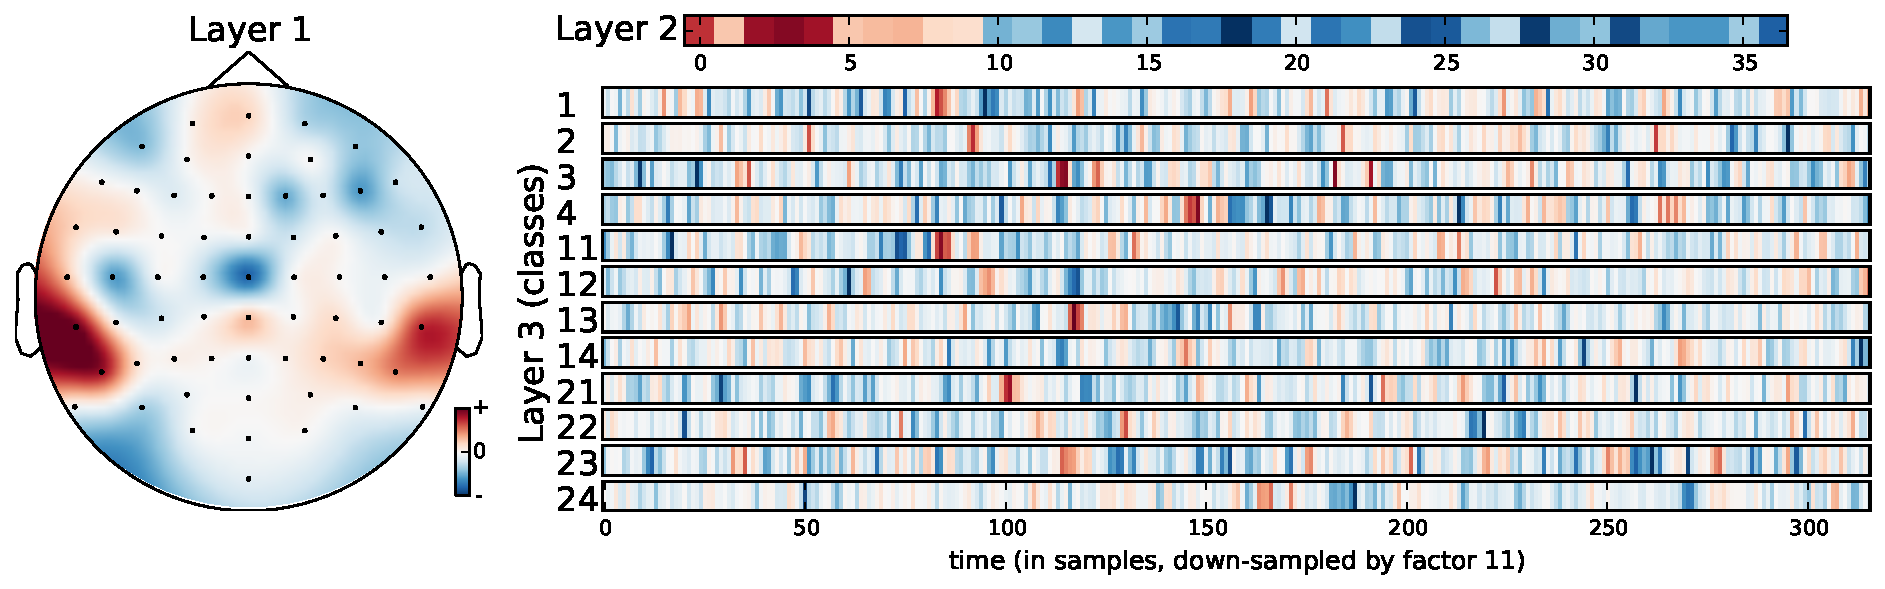
\includegraphics[width=\textwidth,keepaspectratio=true]{Figures/model_W}
%   \\\vspace{-0.8em}
    \caption{Visualization of our neural network, which processes raw EEG at a sampling rate of 512\,Hz.
    Layer 1 was pre-trained using similarity-constraint encoding and is a spatial representation of EEG electrode weights. Layer 2 is a 37 sample long temporal filter. Layer 3 shows the compressed representations of the raw EEG data. The numbers are the ID numbers of the stimuli found in \autoref{tab:stimuli_information}. The colours are an indication of the weighting decided on by the model. We can interpret the intense red and blue colours as being more important for stimulus classification than the white areas.}
    \label{fig:model_W}
  \end{center}
%  \vspace{-1em}
\end{figure}
\section{Layer 2: Temporal Filter \& Layer 3: Templates}
Layers two and three were trained together with supervised learning and optimized by backpropagation through the entire model with a cost function to minimize classification error.
The single data stream output from layer one entered the second layer where it was processed the filter and pooled with a subsampling factor of 11.
This produced a compressed representation of the original EEG data.

To find the optimal parameters (learning rate, filter size, etc.) for our neural network, we employed a 9-fold cross validation scheme by training on the data from 9 subjects (384 trials) and validating on the remaining subject (48 trials).
The cross-validation was done within the training set. %This process created optimized, compressed representations of the EEG data for each stimuli.
The final versions of layer 2 and 3 seen in \autoref{fig:model_W} are an average of the model parameters over all 9 folds.
Layer 2 is the filter that processes the data stream from layer 1, and layer 3 is made up of the optimized, compressed representations of the original EEG data for each stimulus.
\section{Full model explanation}
The classification accuracy of the model was then tested with the test set of 108 trials. 
Each trial in the test set was processed by the filters in layer 1 and layer 2. 
The resulting compressed representation (the output from layer 2) of the test trial was compared against each of the optimized representations in layer 3 of the model.
The dot product of the test trial's representation was taken with each of the optimized layer 3 representations.
This produced 12 values (one for each stimulus) that described the similarity of the test trial's representation with each of the optimized representations. 
Using the dot product as a similarity measure, the test trial was given the label of the stimulus whose representation it was most similar to. 